% !TEX root = Thesis.tex
\chapter{Introduction}\label{chap:Intro}

  On VLSI technology, the analog and mix-signal design play important roles on the SoC (system on chip) design. The concept of analog and mix-signal circuit design today commonly uses a hierarchical strategy for performance specification~\cite{CADonAMSIC_GG-ProcIEEE2000} to satisfy design requirement. In the digital domain, EDA tools are well developed today, certainly down to the lower levels of the design flow. Unfortunately, the story is quite different in the analog and mixed-signal design flow. From circuit synthesis to layout generation, analog and mixed-signal circuit design automation still has tremedous room for improvement. In this dissertation, we first address the problems on analog circuit automation from circuit synthesis to layout generation and then propose our solutions. In this chapter, the problems of analog design automation is generally broken down into three subproblems, which are {\it circuit synthesis with performance exploration}, {\it technology and design oriented constraints for layout generation} and {\it design migration for hierarchical analog circuit}. Section~\ref{sec:overview} enlightens the overview and Section~\ref{sec:contribution} proposes our contributions in this dissertation. 

  \section{Overview}\label{sec:overview}

    In this section, 3 kinds of circumstances in analog design automation are raised. We give an overview of them and show the state-of-the-art. 

    \subsection{Analog circuit synthesis with performance exploration}\label{subsec:PAGEOverview}

      Nowadays, analog circuit block in a SoC design is often critical. Analog components are heavily influenced by nonlinear physical effects, which creates a great barrier for analog automation. Overall, the analog synthesis process consists of topology generation~\cite{TopoSel_ICCAD2008,IPTopoSel_TCAD1995,CAFFEINE_DATE2005}, circuit sizing~\cite{MARS_TCAD2012} and layout synthesis. As topology generation are fully illustrated in~\cite{TopoSel_ICCAD2008,IPTopoSel_TCAD1995,CAFFEINE_DATE2005}, the circuit sizing methodologies also take the indispensable role. Comparing to digital system, the development for analog design automation is still in development. Both topology selection and circuit sizing methodologies are considered in time complexity and the accuracy caused by process variation, parasitics effect and operation conditions.

      There are plenty of works which are already well-developed on how to find optimal design parameters for a prior selected topology. However, as many performance specifications need to be considered, finding the optima solution for multi-objective performance at sizing stage as a priori problem is still uncertain. It seems that deterministic optimization for circuit sizing still has space to improve. Since deterministic optimization keeps the efficiency and full-circuit SPICE-based simulation maintains the accuracy, selecting methodology for analog circuit sizing is beyond trade-off. 

      Therefore, in order to explore the limitation of targeting technology, having an efficient multi-objective synthesizer is essential. Moreover, it should also be capable of searching the performance space and mapping to design parameters with accuracy and efficiency for analog circuit design perspectives.

      \subsubsection{Previous Works}
        State-of-the-art analog synthesis methodologies were formulated as a numerical problem which relies on macro-modeling. Usually a complete circuit schematic and the circuit's performance spec are given, then the sizes and biasing value of all devices have to be determined. As a result, the optimal values meet the specs of the required circuit. This kind of optimization engine determines these optimal values and there exists an evaluation engine to assess the performance. It is very likely that the initial sizing result in a near-optimal design, therefore, a further fine-tuning follows for improving yield and design robustness~\cite{HierModeling_ProIEEE2007}. 

        In algorithm of \cite{Simu_DATE2000}, a numerical simulation has been employed successfully, while deterministic optimization are developed in \cite{MARS_TCAD2012,Habal_TCAD2011}. At the same time, methods to acquire accurate yet interpretable analytic formulation as design equations in posynomial forms have been proposed intensively in~\cite{PWL_Convex_GP,Eeckelaert_DATE2003}. Analog/RF design problems can be described as posynomial form in order to be fed as standard input for convex optimization problem. Thus, the convex problem is certainly solved efficiently with accurate design equation~\cite{Device_CKT_CoOpt_GP}. These approaches attempt to generate the mapping from device models to performance metrics, and then utilize the numerical solvers or optimization engines to re-target the corresponding device-level parameters. Although the process of such limited-scaled device modeling is efficient and accurate, the circuit design equations are imprecise and hardly express the global nonlinearity. Another kind of approach~\cite{RobustPosyMdl_ICCAD2004,PerfCentOpt_ICCAD2005} shows that the performance space can be modeled in posynomial form for system-level design and trade-off analysis. It directly maps the device-level design variables to performance metrics. Such approach can improve the precision but requires iterations on time-consuming full-sized circuit simulation for optimality. However, it restricts to small-scaled circuit since the execution time depends on the circuit complexity, and usually grows exponentially. 

        In all, due to the requirement for more probability on performance metrics, we believe that it is important to have mechanism at the early design stage in exploring the performance limitation before optimization. Meng et al.\cite{PerfMap_ISQED2011} provides a hierarchical performance Pareto-front mapping methodology to acquire performance metrics before circuit optimization stage. \cite{PerfMap_ISQED2011} first traverses the performance specs as constraints in a set of convex problem. Therefore, a combination of performance space is generated. Moreover, the corresponding design variables can be obtained according to the design equation. Labrak et al.~\cite{HybridOpt_MWSCAS2007} performs a hybrid optimizer with a multi-objective optimization problem(MOOP) for a CMOS Op-Amp. Our method integrates the hierarchical synthesis strategy with a performance mapping methodology and a non-uniform circuit simulation approach to meet the multi-objective performance requirement wisely. 

    \subsection{Technology and design oriented constraints for layout generation}\label{subsec:HCDROverview}

      The analog layout design should follow process rule and design description to fulfill the analog physical design. However, the problem in layout generation is not as easy as a simple geometrical problem since the layout characterization such as placement and routing status directly affects the performance of the required circuit design. Most of the time, the modification is critical through some inter-die correlations which bring the most significant parasitics and matching behavior. Therefore, this area has been one of the most studied areas in analog design automation. 

      It is simple for process of analog layout automation to apply the best topology from manual schematic views of circuit design~\cite{ALE-iscas1990}. The device diagrams in circuit-level can be replaced with parametrical (or programmable) cells which are created by PDKs (process design kits). PDKs mostly are provided by foundries to support full custom design flow. Since the circuit designer can annotate relationships among devices on the schematics, these relationships are taken into account at the placement phases. In~\cite{apnsi-pohung-dac07,mscgrlal-tcad2006Jun} and~\cite{palpndg-iccad2011}, devices relationship topology can also be extracted from template designs to generation placement results. After placement, the routing algorithm is performed to check for design verification. At this stage, when practical implementation on advance technology nodes such as 40nm, it is necessary for routing strategy to be aware of process rule efficiently. Hence, The placement topology should be retained to the routing stages. Thus, our method tends to focus on both the prior-stage controllability for routing characteristic and layout-dependent-effect(LDE) at analog routing automation. 
      \subsubsection{Previous Works}
        The analog routing problem considering various constraints has been addressed in the literature. The first router~\cite{anrmfca-CICC1990} which takes constraints into account claims that a simple cost function consisting of wire length and parasitics effects is not realistic. This router shows a routing problem as a grid-less and symbolic routing, and a detail routing procedure is performed with net ordering technique. In~\cite{GeneralRouter-CompEuro89}, Malavasi et al. utilizes a scheduler for net-ordering on a maze router. Nonetheless, the router is improved in~\cite{sensitAR-iccad90} to traverse the sensitivity of the critical parasitics and user-defined priorities. The authors also provide the way to partition nets with different current densities~\cite{arearouting-tcad1993}. In another approach~\cite{GRforAMS-SOCC2001}, multiple routed candidates are generated for each net. Thus, the candidate routes can be specifically selected according to each performance requirement. In KOAN/ANAGRAMII~\cite{KOAN_ANAGRAMII-JSSC1991}, Cohn et al. merges individual devices to macrocells by abutment to achieve dense layout other than adding explicit wires. Moreover, ANAGRAMII practices over-the-device wiring and allows RRR (rip-up and reroute) for more flexibility. Recently, topic on shield routing~\cite{shieldRouting-islped2010} has been implemented based on net classification for optimal area shielding. For routing matching problem, Ozdal et al. propose a dynamic programming approach to resolve~\cite{AnalogRouteMatching-iccad2009}. In~\cite{LinfuXiao-iccad2010}, Xiao et al. also claim that the symmetrical routing can be achieved by routing one part of a symmetric group at first, and then the counterpart is generated by mirroring the previous one.
        
        \begin{figure}[ht]
          \centerline{
            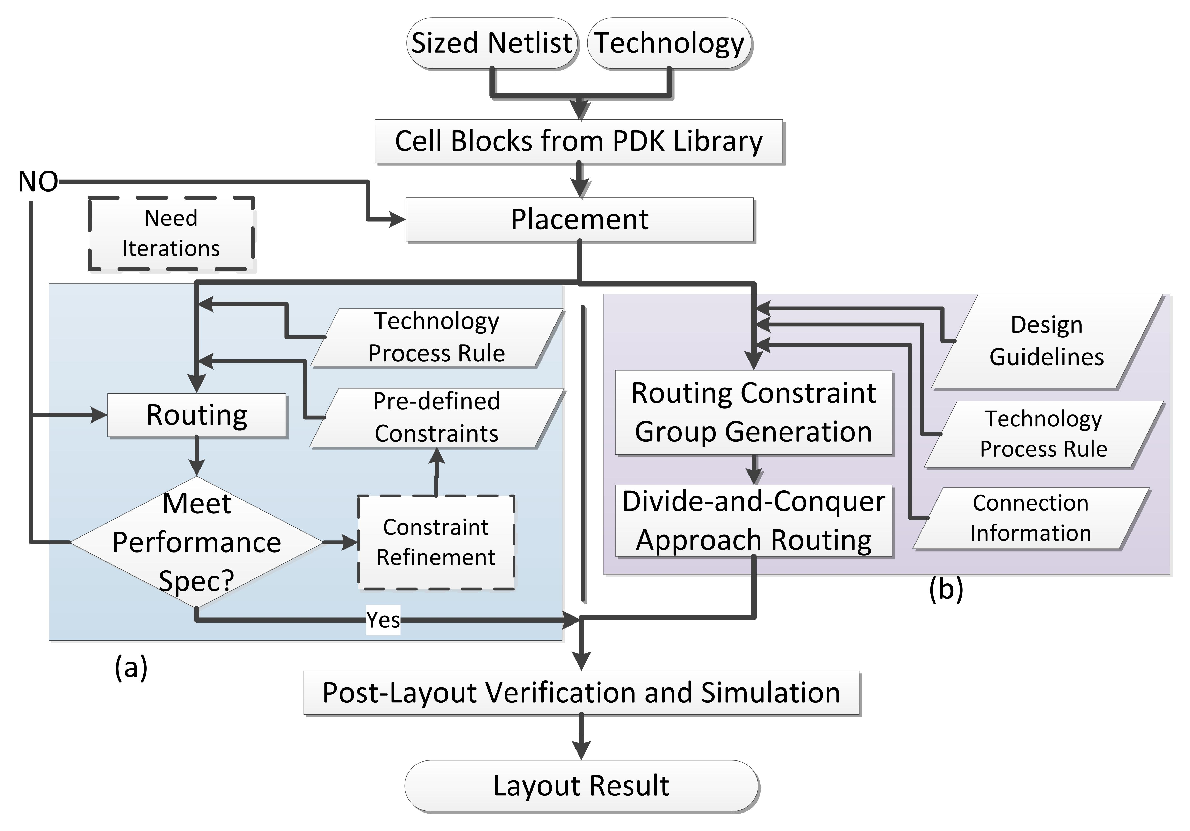
\includegraphics[width=0.7\textwidth]{Fig/Introduction/LayoutFlow.eps}
          }
          \caption{Two analog layout general flow. (a) traditional routing with pre-defined constraints. (b) Our approach with routing constraints generation. }
          \label{fig:LayoutFlow}
        \end{figure}
        Most of the previous works show great effort on resolving analog routing with application-defined constraints on their own algorithms, such as~\cite{anrmfca-CICC1990,sensitAR-iccad90} and~\cite{arearouting-tcad1993}. However, the spirit of analog layout design is to preserve the know-how design constraint information from circuit-level designers to experienced analog layout designers. Since a series of simple objectives for placement/routing strategy on analog layout is conceptually impractical, the layout design from automation methodology is far from the expectation eventually. In order to honor analog designers' experience, a general constraint unification among transistor-level and physical-level is essential. Beside the design objectives, the physical design rules from advanced technology are grown in exponential complexity. Due to the issue of design for manufacturability(DFM), the simple constraints such as layer spacing, layer enclosure and minimum width cannot cover the process rules completely. For analog design, the restrictions should be more conservative for accurate performance. The hierarchy is introduced in \cite{phLin-dac2008} and \cite{ymYang-isqed2010} for analog design automation. However, Lin et al. in \cite{phLin-dac2008} utilize hierarchical module only for placement and Yang et al. in \cite{ymYang-isqed2010} build a hierarchical constraint tree, which is actually a tree style constraint map focusing on global routing purpose. According to design and process issues, a collection of constraints which can simultaneously resolve process rules and design conditions is needed by automated layout engine. Moreover, the constraints should guarantee the extensibility for advanced technology and flexibility for various design purposes.   

    \subsection{Design migration for hierarchical analog circuit}\label{subsec:DMOverview}
      
      As the complexity of the advanced nodes for analog circuit increases, the layout constraints and the expanding performance requirements become major productivity bottlenecks. Lately, in order to alleviate the impact from process variation beyond the transistor level as well as striving for excellent performance, analog layout design mostly relies on designers' expertise. However, the iterative refinement on manual design damages the productivity of analog layout. Other than just manipulate schematic and layout constraints manually, it is more efficient to enroll the know-how from existing designs instead of generating a new one. To migrate layout template via preservation becomes a plus.

      For analog layout, reusability relies on the similarity such that part of source layout can be reused to add new modules or layers on target layout with trivial modification. To preserve the design knowledge from the template layouts, the devices' relative positions and the routing behaviors should be considered thoroughly. Typical analog constraints such as symmetry and proximity constraints fundamentally regulate the placement. On the other hand, wire symmetry and topological matching are critical to analog routing. Placement and routing extracted from the template layout can benefit layout migration. In other words, more informations are extracted from template layout, more circuit characteristics are preserved. Currently, analog layout preservation pays more attention on placement~\cite{cart-hammouda-dac06,cbc-bhattacharya-dac04,Wang_ALRGP_TODAES2011} for topology extraction. However, seldom do we study routing behavior extraction in previous works. In all, a solution to preserve the correlation during layout retargeting, or so-called layout migration is critical.

      \begin{figure}
        \centering
        \begin{subfigure}[t]{0.4\textwidth}
        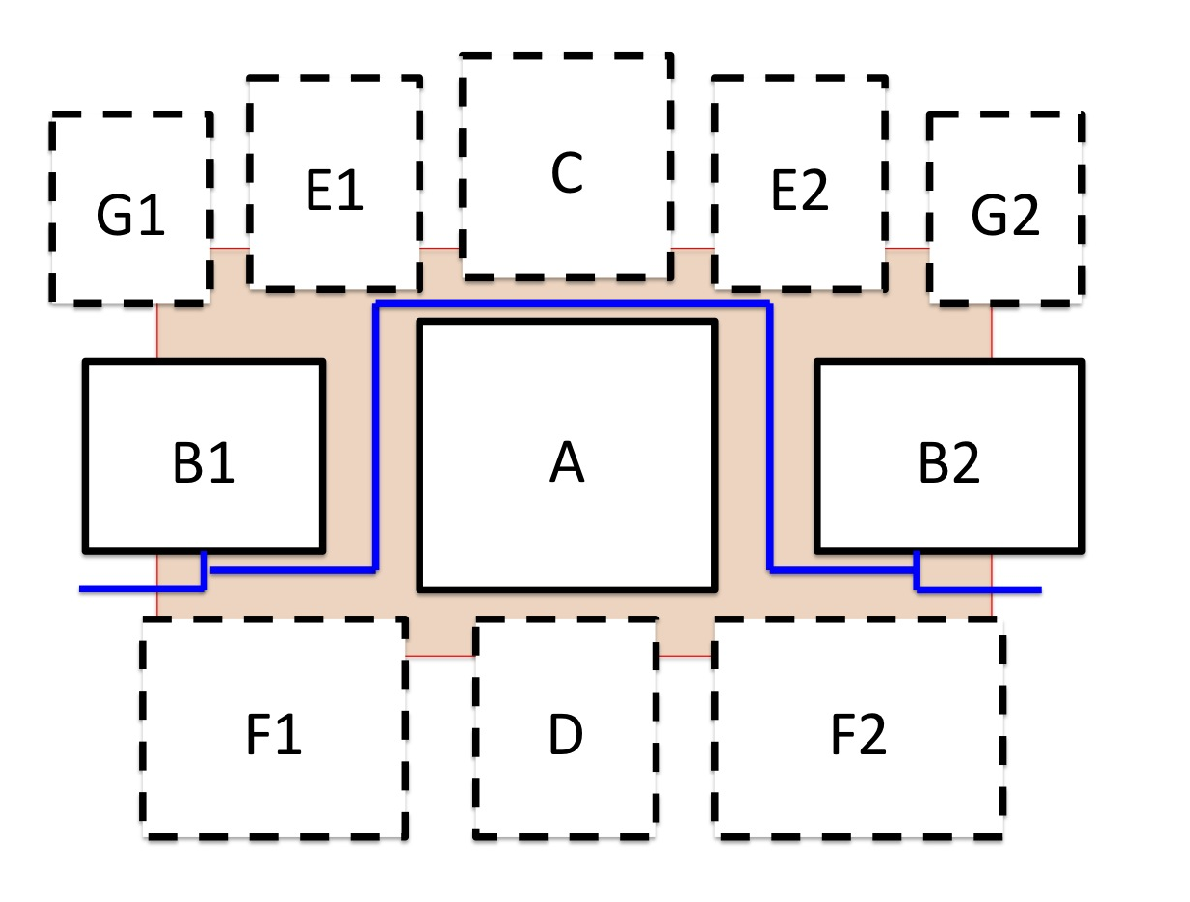
\includegraphics[width=\textwidth]{Fig/RoutingPreserv_a.eps}
        \caption{Reference template layout}
        \label{fig:RoutingPreserv_A}
        \end{subfigure}
        \begin{subfigure}[t]{0.4\textwidth}
        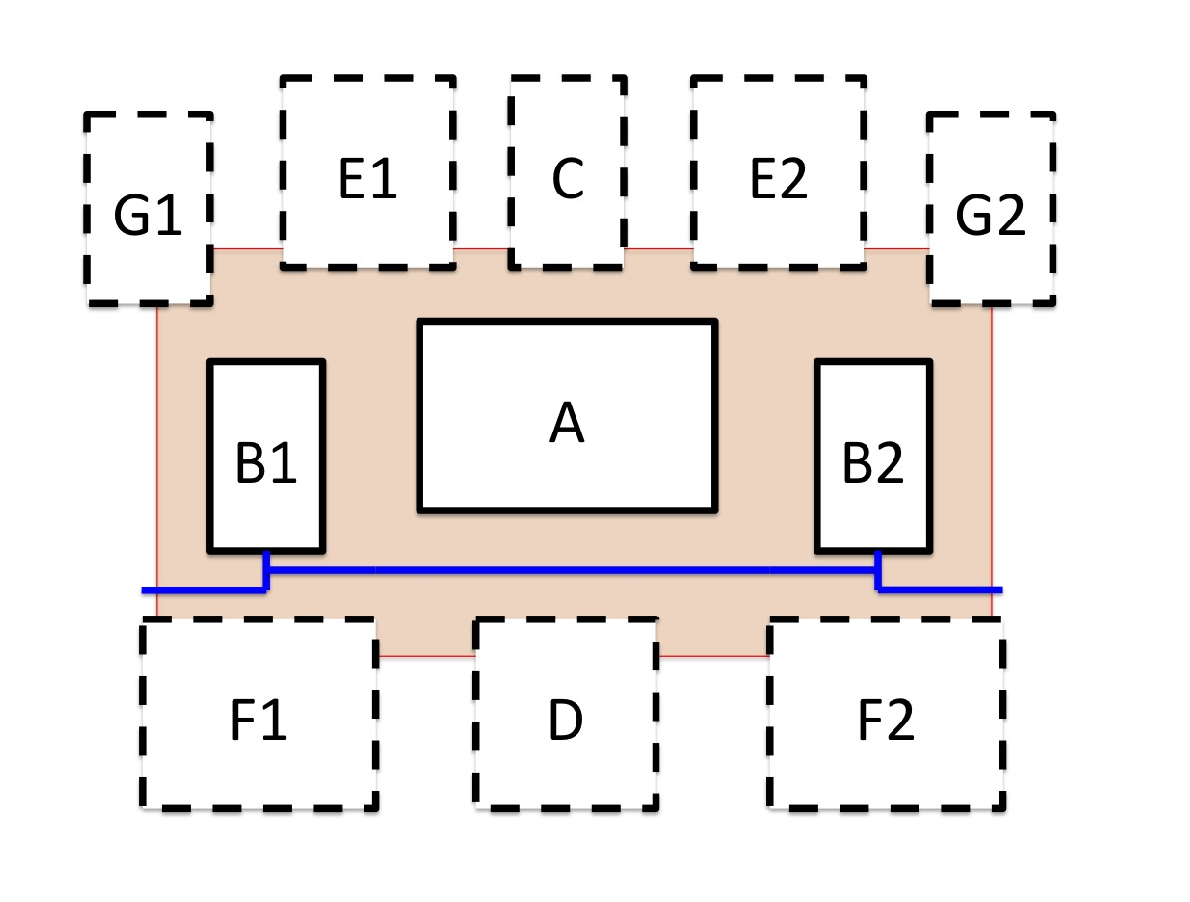
\includegraphics[width=\textwidth]{Fig/RoutingPreserv_b.eps}
        \caption{Non-preserved automatic routing}
        \label{fig:RoutingPreserv_B}
        \end{subfigure}
        \begin{subfigure}[t]{0.4\textwidth}
        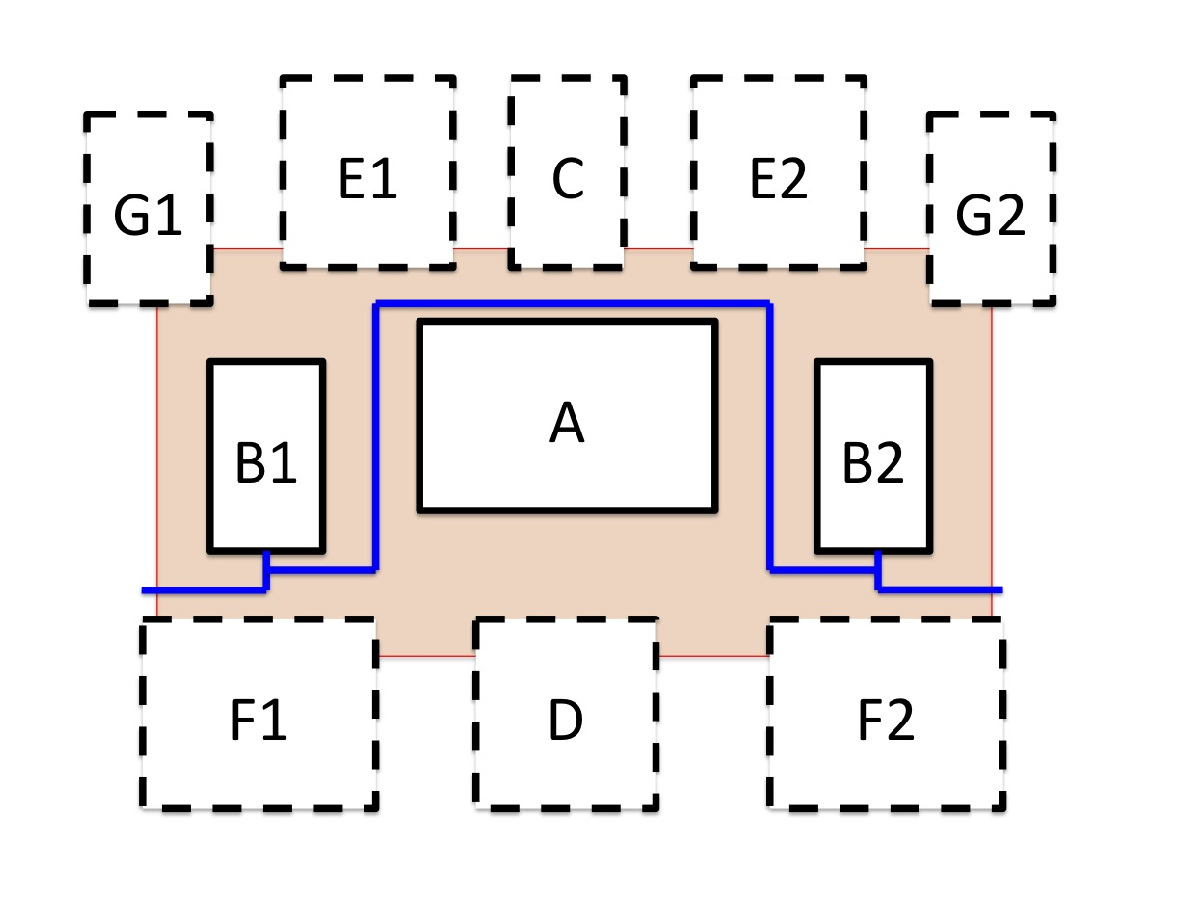
\includegraphics[width=\textwidth]{Fig/RoutingPreserv_c.eps}
        \caption{Preserved routing}
        \label{fig:RoutingPreserv_C}
        \end{subfigure}
        \begin{subfigure}[t]{0.4\textwidth}
        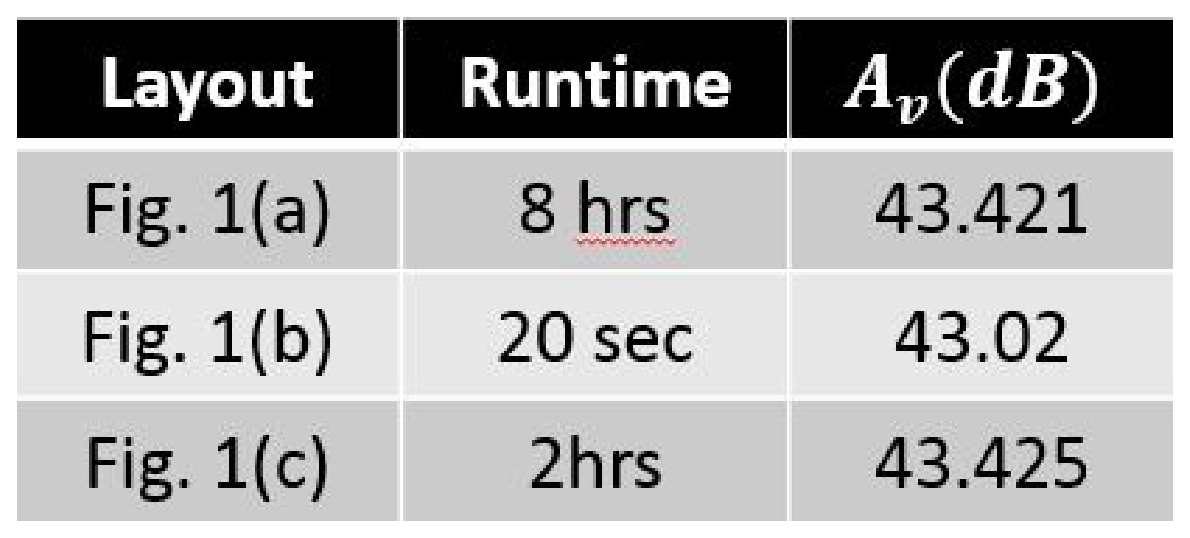
\includegraphics[width=\textwidth]{Fig/RoutingPreserv_d.eps}
        \caption{Timing and simulation results}
        \label{fig:RoutingPreserv_d}
        \end{subfigure}
        \caption{Analog layout generation with different configuration. (a) Reference layout with complete placement and routing. (b) non-preserved automatic routing considering usual constraints only. (c) layout generation considering preserved routing characteristics. (d) simulation results in umc65nm technology.}
        \label{fig:RoutingPreserv}
      \end{figure}

      A simple experiment shows the necessity of routing preservation. In Figure~\ref{fig:RoutingPreserv}, we compare the analog layout generation with two configurations. Figure~\ref{fig:RoutingPreserv_B} automatically generates analog layout with respect to analog constraints only, and Figure~\ref{fig:RoutingPreserv_C} keeps more preserved routing informations from the reference layout in Figure~\ref{fig:RoutingPreserv_A}. Even though the routing path in Figure~\ref{fig:RoutingPreserv_C} from $B1$ to $B2$ is detoured in the reference layout, the simulation result obviously shows that it earns better performance than Figure~\ref{fig:RoutingPreserv_B} on voltage gain over 0.4$dB$, which makes the path straightly connecting across the tunnel between $A$ and $D$. Under the same configuration of circuit sizing, these two layouts represent the performance response of reusability. According to the original perspective of design, the detour benefits the parasitic effect of the intersection on wires. Besides the performance result, we also observe that the runtime of Figure~\ref{fig:RoutingPreserv_C} is remarkably improved than Figure~\ref{fig:RoutingPreserv_B}. 
      
      There are more layout generation experiments illustrated in Section~\ref{sec:RLPADMExp}, and these experiments show that automatically generated layouts with preserved information have superior performance. Meanwhile, the preserved information represents the routing behavior extracted from the original layout. By applying the preserved routing behavior, it can produce the migrated layout more efficiently than manually migration. As a result, migration with preserved information facilitates the flow of layout generation, that reduces the time-to-market. In other words, the productivity is raised.

      \subsubsection{Previous Works}

      The problem of layout retargeting has been widely discussed in the literature. We can roughly categorize them into two major stages, placement and routing. At the placement stage, certain approaches mainly focus on fully mapping~\cite{Bhattacharya_ASPDAC04,cbc-bhattacharya-dac04,msc-bhattacharya-tcad06,Zhang_TCAD08,LayoutRetarg_Liu_ASPDAC2010,Wang_ALRGP_TODAES2011}. First of all, Bhattacharya et al. in~\cite{Bhattacharya_ASPDAC04} detect the symmetric components from the source layout hierarchically and retarget it. \cite{cbc-bhattacharya-dac04} later enhance the retargeting layout with compaction. Hammouda et al. in\cite{cart-hammouda-dac06} combine the device resizing, layout compaction as a full layout retargeting flow. In \cite{msc-bhattacharya-tcad06}, Bhattacharya et al. extend the compaction to larger analog design as the multi-level layout generation. Moreover, in \cite{Zhang_TCAD08}, Zhang et al. deal with the parasitic effects as well as retargeting the compaction-based layout. Wang et al. build template for analog layouts and then use geometric programming to guarantee the global optimal solution for compaction in \cite{Wang_ALRGP_TODAES2011}. 

      Since compaction holds almost the same topology from the source layout, it constructs a symbolic structure to preserve layout topology, technology rules, symmetry and proximity constraints. Additionally, Weng et al. in~\cite{ALP_YPWeng_iccad2011} provide prototypes with Defer~\cite{defer_jackey_tcad10} in migrated layout due to the different scale ratio among devices efficiently. Method in~\cite{ALP_YPWeng_iccad2011} successfully reduces the white space under target technology and obtains better performance after post-layout simulation. 

      For routing, the existing researches rely more on routing generation with constraints rather than retargeting. Early works in~\cite{KOAN_ANAGRAMII-JSSC1991,aicon_malE_tcad96,ppraic_Linfu_iccad2010} propose a maze-style router in order to consider symmetry and non-symmetry modules in the same design. Channel routing is also adopted by~\cite{cbcrams_UChoudhury_tcad93} and \cite{aicon_malE_tcad96} to deal with mirror symmetry and detailed routing among blocks. Recently, other than symmetry issue, exact matching constraints for maze routing are well addressed in ~\cite{ermams_MMOzdal_tcad09}. Ou et al. in \cite{numarmc_HCOu_dac12} first define three typical matching constraints for analog routing which dominates performance most: {\it(1)symmetry, (2)topology-matching} and {\it (3)length-matching}. 

      Additionally, Pan et al. in \cite{Pan_CGR_ICCAD2012} claim that routing priority considering constraint group in hierarchy can enhance the signal integrity. Still, work in LAYGEN II \cite{LAYGENII_TCAD13} performs an evolutionary multi-objective way to evaluate an optimized routing results from layout templates. Lately, \cite{SAPR_DAC13} proposes a simultaneous analog placement and routing framework which further considers the current flow constraints for critical nets. Overall, although the symmetry and matching constraints are well treated and routing matching constraints are extended further, the correlation among wires and placement has not been systematically preserved as a guideline to migrate.

  \section{Our Contributions}\label{sec:contribution}
    \subsection{Parallel genetic performance exploration for multi-objective analog circuit synthesis}

      \begin{figure}[ht]
        \centerline{
        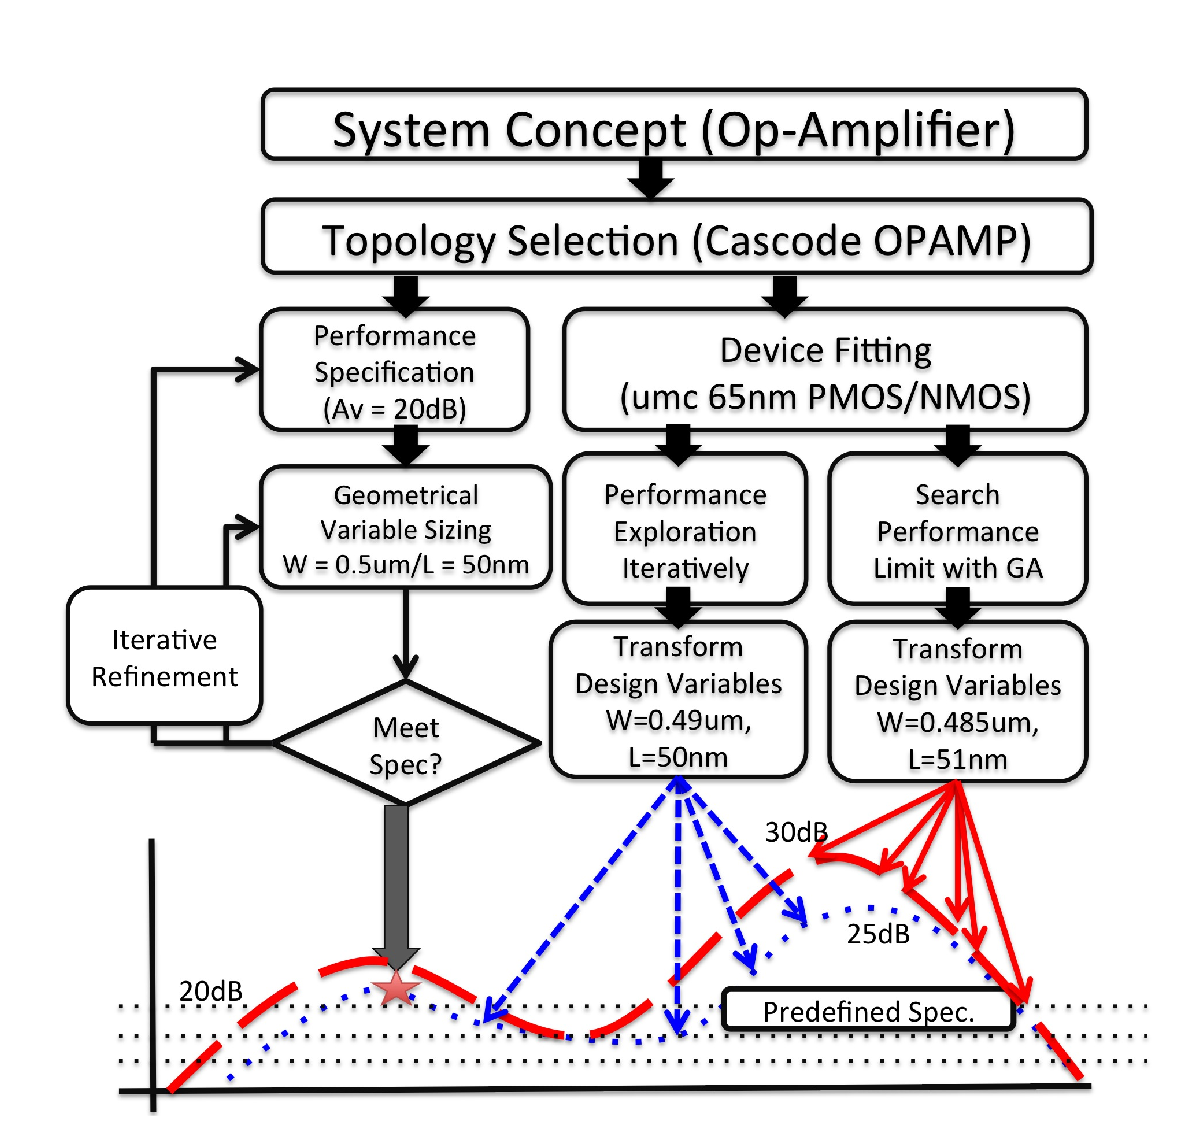
\includegraphics[width=0.7\textwidth]{Fig/Introduction/PerfCons.eps}}
        \caption{While traditional sizing strategy iteratively searchs the solution beyond the fixed spec, a performance constraints exploration approach unfolds the utmost of performance space. Moreover, an evolutionary methodology application elaborates exploration faster and more precise.} 
        \label{fig:PerfOptimal}
      \end{figure}

      Generally speaking, it is rarely possible to find an optimal solution for all performance requirements in advanced nodes. Therefore, it is practical to search the performance limitation with agile and accurate synthesis procedure. Referring to~\cite{PerfMap_ISQED2011}, Meng et al. attempt to search the performance space by re-targeting back to the corresponding design variables, in iterative manner. Nevertheless, the strategy which costs time complexity up to $O(S^K)$(S stands for the performance range in discrete number and K represents the number of performance specification), which is time-consuming and will lose the effective prediction of performance metrics. To our best knowledge, genetic algorithm is well developed for many analog synthesis topics in \cite{DARWIN_DAC1995,CAFFEINE_DATE2005,HeteroSyn_DATE2006,NominalYieldArea_AHS2009}. On the contrary, the proposed research employs a parallel genetic algorithm (PAGE) for traversing performance space as optimization constraints. A parallel genetic algorithm like \cite{SurveyPGA1997,SurveyDistPGA1997} can divide the target population into several sub-populations with particular performance specs and reunion after evolution. The obtained populations resulted from PAGE can be re-targeted to the non-uniform stochastic circuit simulation. Figure~\ref{fig:PerfOptimal} illustrates the comparison among the traditional optimization on performance specification, the iterative performance exploration by~\cite{PerfMap_ISQED2011} and our methodology with novel parallel genetic algorithm engine. The proposed research achieves three principle contributions as follows: 
      \begin{itemize}
      \item {\bf Hierarchical synthesis architecture.} This synthesis demonstrates a bi-direction search approach for device model fitting to performance metrics through circuit-level domain. After obtaining the corresponding performance space, it re-targets to feasible device level design parameters with a good prediction.
      \item {\bf Parallel genetic algorithm based multi-objective performance exploration}. A multi-objective evolutionary methodology like parallel genetic algorithm (PGA) not only performs evolution in parallel for diverse performance metrics, but also migrates chromosome by interleaving among populations. PAGE brings out a population of potential solution for selected performance among metrics. Such population is also projected to the feasible design parameters so that we affirm the global optimal solution is located nearby this optimization result by exploration.
      \item {\bf Probabilistic circuit simulation.} The performance space not only stands for the potential optimum, but also represents the possibility of suitable design parameters which cause better performance. This dissertation integrates each design variable to analyze the possibility distribution. Other than uniformly swapping the values of design variables in stochastic searching, an interval with higher possibility earns more searching resources. A nonuniform step searching for circuit SPICE simulation is proposed.
      \item {\bf Experimental results with RFDA and two-stage operational amplifier} show that our hierarchical synthesis framework can efficiently trace the optimal solution for analog circuits. First of all, we compare the performance exploration approach between parallel and non-parallel genetic algorithm. Then we compare the perturbation stage with uniform and probabilistic simulation. The simulation results also show that our integration can satisfy higher performance than the previous work.
      \end{itemize}

    \subsection{Configurable constraint-driven analog routing}

      In this paper, we present a hierarchical constraint driven routing methodology. This methodology determines the analog routing order by the hierarchical constraint groups. Such constraints preserve both the objective physical technology constraints and the subjective  analog design-oriented constraints. Other than adopting the self-defined constraints for routing, this dissertation provides an innovative uniform constraint group for routing. Such constraint group is based on uniform OpenAccess constraint group model and contains both foundry level process rules and analog design-knowledge constraints. By maintaining the universal industrial constraint format, it is feasible for different placement-and-routing engines to co-design by accessing the same constraint group for consistency. This dissertation first presents a constraint group generation for analog layout design with a selected technology. We then practice the hierarchical constraint-aware routing decision flow in a divide-and-conquer approach. The overall framework is illustrated in Figure~\ref{fig:LayoutFlow}. 
    

      As Figure~\ref{fig:LayoutFlow} shows, most of previous methodologies attempt to apply self-defined constraint format. Unlike such traditional scenario, our framework aims to have the following characteristics :
      \begin{itemize}
        \item {\bf An extensible universal constraint semantic.} We generate the general format for analog constraints which is extendible for describing advanced technology rules. Also, the flexibility of OpenAccess constraint group assists this methodology to preserve the analog circuit characteristics at the prior stage, such as placement-level even schematic-level.
        \item {\bf A hierarchical constraint group generator.} The analog design constraints such as symmetrical and matching properties are integrated into a hierarchical constraint group, in which the priority of constraints dominates the order of modules to be routed.
        \item {\bf A guided constraint-driven router.} For the sake of keeping signal integrity at the routing stage, our strategy performs a guided router which can determine the order of nets referring to designer's expertise and the LDE.
      \end{itemize}

    \subsection{Rapid migration framework via prototyping and wire segment refinement}

      While the aforementioned mechanisms in section~\ref{subsec:DMOverview} successfully facilitate layout migration with designers' know-how on placement, the behavior of routing has not been extracted essentially. Thus, the template-based layout migration does not benefit routing much. 
 
      In addition, the routing generation relies on automatic routing methodologies with respect to the placement constraints. Such constraints in ~\cite{cbc-bhattacharya-dac04,Bhattacharya_ASPDAC04,msc-bhattacharya-tcad06,Zhang_TCAD08,Wang_ALRGP_TODAES2011} are not suitable for routing generation. 

      In Chapter~\ref{chap:RLPADM}, we propose an analog layout migration flow with the best preservation that rapidly generates the analog layout on the target technology. We briefly sum up our contributions as follows:

      \begin{itemize}
        \item {\bf A bottom-up prototyping framework for analog layout migration} is delivered. According to the information extracted from the existing layout, the full layout with placement and routing can be migrated automatically with high reusability. Works in \cite{ALP_YPWeng_iccad2011} and \cite{Chin_DMR_ICCAD2013} migrate placement and routing from template layout separately. However, the correlation among placement and routing is inalienable. This dissertation proposes a multilevel migration framework which simultaneously reduces the redundancy of routing as well as achieving the qualified circuit performance.
        \item {\bf A wire refinement methodology} is proposed to further improve performance metrics right after the routing settled. Given the target technology design rules, placement, wires and pin connection information, it is sufficient to explore the optimization of the width of wires.
        \item {\bf A fast multiple analog layout generator} illustrates that our prototyping framework is capable of producing routing results with different topologies from the source layout. The resultant layouts show that our representation realizes multiple layouts efficiently.
      \end{itemize}

      Current layout migrations limit the flexibility of routing reconstruction. This work achieves effective and adjustable layout retargeting. Yet, it allows designers to decide the relevant solution from multiple candidates. Some of previous results were presented in \cite{Chin_DMR_ICCAD2013}. Instead, this work appreciates the comparison with state-of-the-art.

  \section{Organization of this dissertation}\label{sec:organization}
    In this dissertation, Chapter~\ref{chap:Intro} first introduces the problems of the analog design automations among circuit synthesis, constraints integration and layout generation, and then proposes our contributions in this dissertation. Chapter~\ref{chap:PAGE} presents an analog circuit synthesis via genetic performance exploration, whose goal is to fast explore the limitation of performance in different technologies of integrated circuit. Chapter~\ref{chap:CUCLM} introduces an unification of technology and design constraints for analog design to manipulate constraint-driven routing efficiently. A rapid migration framework of analog circuit design is detailed in Chapter~\ref{chap:RLPADM} via layout prototyping, which considers both placement and routing during layout extraction. Furthermore, this migration flow also refines wire segments before signed-off. Finally, Chapter~\ref{chap:CFW} draws the conclusions and future works.
